\documentclass[10pt]{article}
\usepackage[paperwidth=198mm,paperheight=59mm,margin=1mm]{geometry}
\usepackage{newtxtext,newtxmath,tikz,pgfplots}
\pgfplotsset{compat=1.18}
\definecolor{methodblue}{HTML}{216A85}
\definecolor{controlgray}{HTML}{555555}
\definecolor{accentorange}{HTML}{A64B1D}
\pagestyle{empty}
\begin{document}\noindent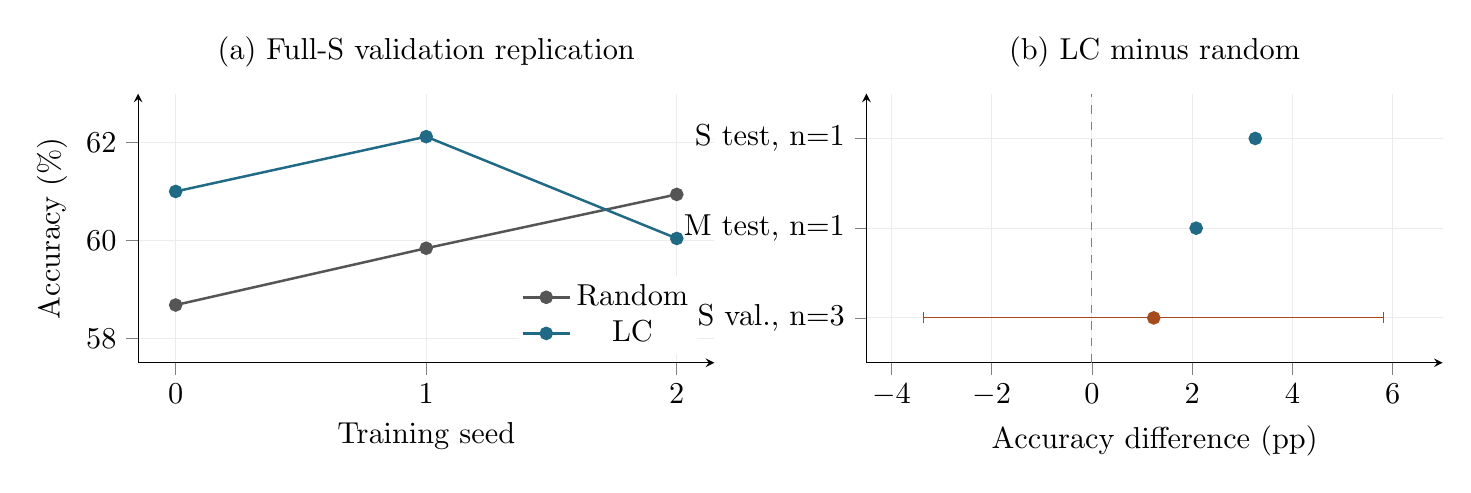
\begin{tikzpicture}
\begin{axis}[width=89mm,height=50mm,axis lines=left,tick align=outside,grid=major,grid style={gray!15},scaled ticks=false,tick label style={font=\fontsize{11}{13}\selectfont},label style={font=\fontsize{11}{13}\selectfont},title style={font=\fontsize{11}{13}\selectfont},legend style={font=\fontsize{11}{13}\selectfont,draw=none,fill=white,inner sep=1pt},title={(a) Full-S validation replication},xmin=-.15,xmax=2.15,ymin=57.5,ymax=63,xtick={0,1,2},xlabel={Training seed},ylabel={Accuracy (\%)},legend pos=south east]
\addplot+[color=controlgray,mark=*,mark size=2pt,line width=0.9pt,mark options={solid,fill=controlgray,draw=controlgray}] coordinates {(0,58.68)(1,59.84)(2,60.94)};
\addlegendentry{Random}
\addplot+[color=methodblue,mark=*,mark size=2pt,line width=0.9pt,mark options={solid,fill=methodblue,draw=methodblue}] coordinates {(0,61)(1,62.12)(2,60.04)};
\addlegendentry{LC}
\end{axis}
\begin{axis}[width=89mm,height=50mm,axis lines=left,tick align=outside,grid=major,grid style={gray!15},scaled ticks=false,tick label style={font=\fontsize{11}{13}\selectfont},label style={font=\fontsize{11}{13}\selectfont},title style={font=\fontsize{11}{13}\selectfont},legend style={font=\fontsize{11}{13}\selectfont,draw=none,fill=white,inner sep=1pt},at={(9.25cm,0)},anchor=south west,title={(b) LC minus random},xmin=-4.5,xmax=7,ymin=-.5,ymax=2.5,ytick={0,1,2},yticklabels={{S val., n=3},{M test, n=1},{S test, n=1}},xlabel={Accuracy difference (pp)}]
\draw[dashed,gray] (axis cs:0,-.5)--(axis cs:0,2.5);
\addplot+[color=methodblue,mark=*,mark size=2pt,line width=0.9pt,mark options={solid,fill=methodblue,draw=methodblue},only marks] coordinates {(3.26,2)};
\addplot+[color=methodblue,mark=*,mark size=2pt,line width=0.9pt,mark options={solid,fill=methodblue,draw=methodblue},only marks] coordinates {(2.08,1)};
\addplot+[color=accentorange,mark=*,mark size=2pt,line width=0.9pt,mark options={solid,fill=accentorange,draw=accentorange},only marks,error bars/.cd,x dir=both,x explicit] coordinates {(1.2333333,0) +- (4.5897652,0)};
\end{axis}
\end{tikzpicture}\end{document}
